\captionsetup{justification=centering}
\begin{figure}[H]
    \begin{subfigure}{1\textwidth}
        \centering
        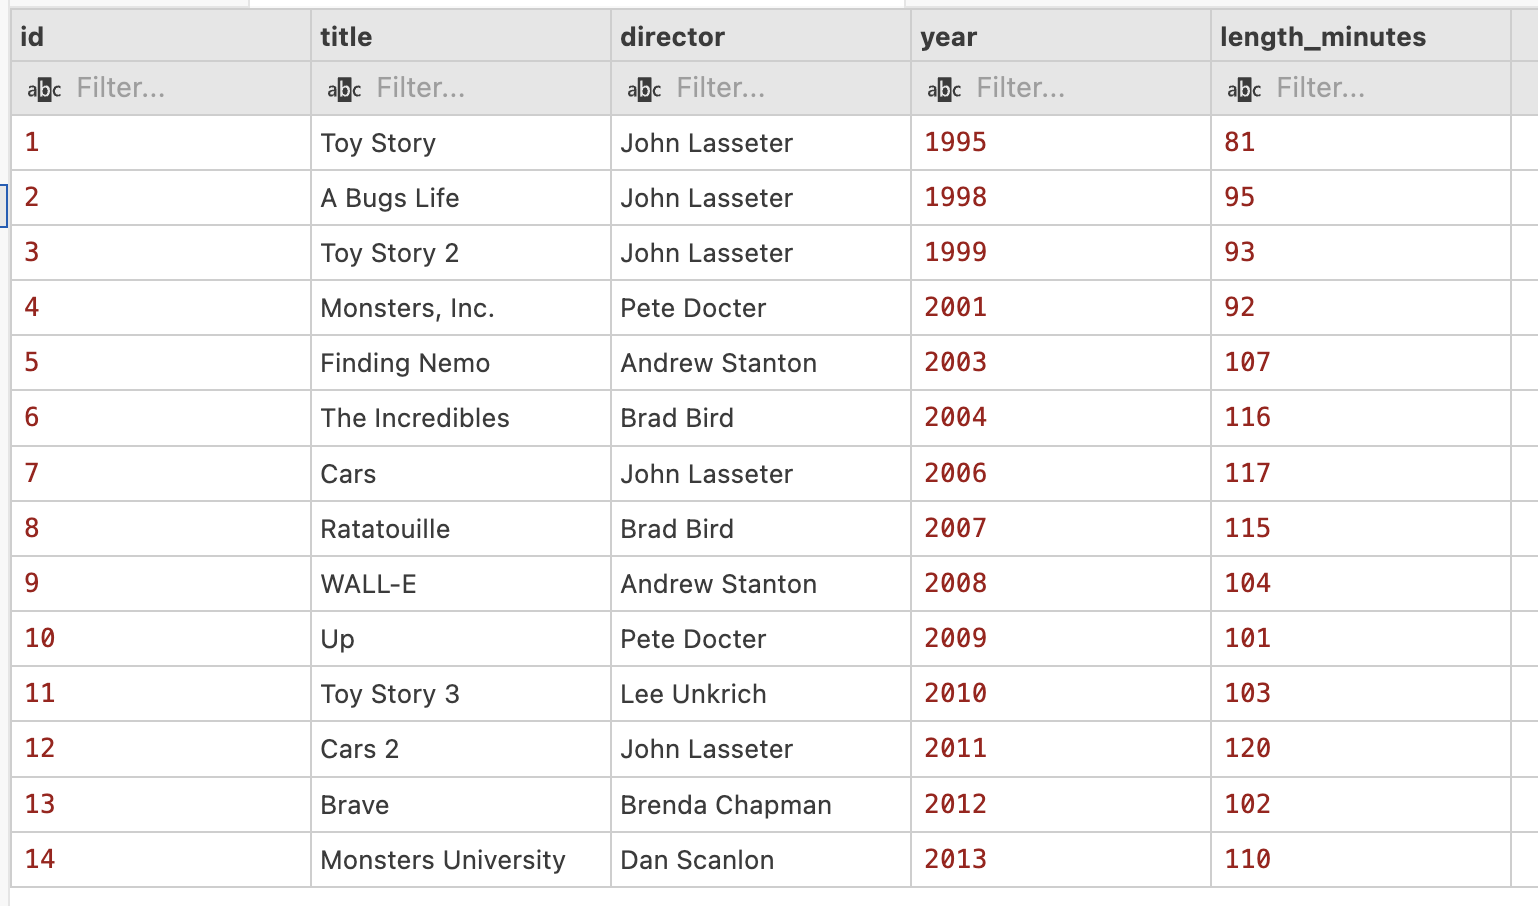
\includegraphics[width=.6\linewidth]{images/output/mov.png}
        \caption*{The complete Movies table.}
        \label{fig:mov}
    \end{subfigure}
    \begin{subfigure}{1\textwidth}
        \centering
        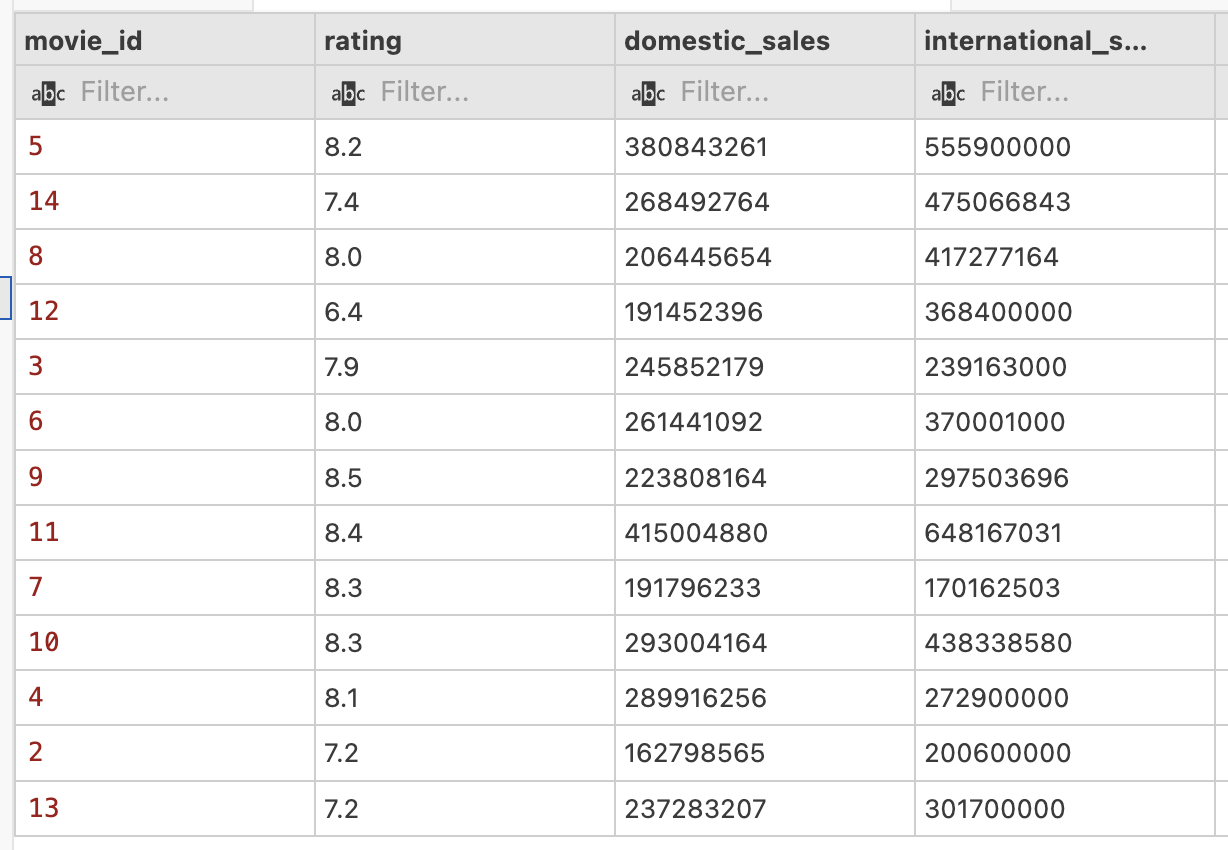
\includegraphics[width=.6\linewidth]{images/output/box.png}
        \caption*{The complete Box Office table.}
        \label{fig:box}
    \end{subfigure}
    \vspace*{10mm}
    \vspace*{10mm}
    \begin{subfigure}{.5\textwidth}
        \centering
        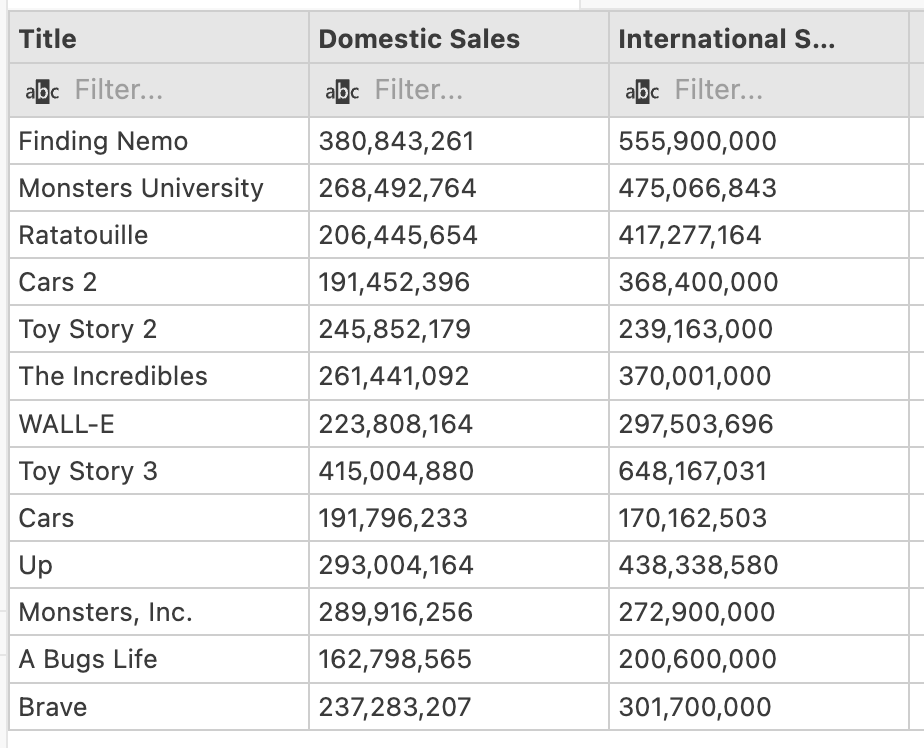
\includegraphics[width=.8\linewidth]{images/output/q5.png}
        \caption*{Domestic \& international sales for each movie.}
        \label{fig:q5}
    \end{subfigure}
    \begin{subfigure}{.5\textwidth}
        \centering
        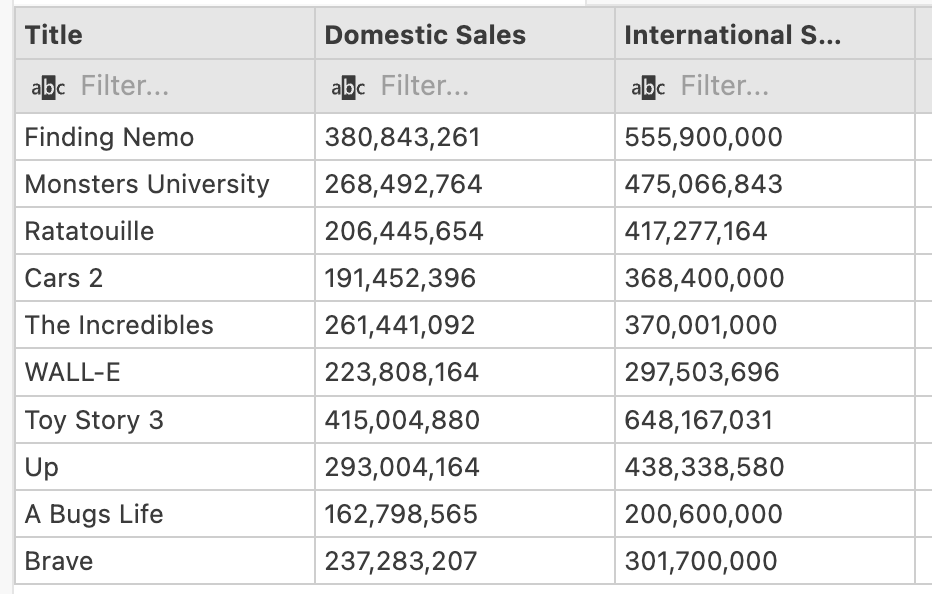
\includegraphics[width=.8\linewidth]{images/output/q6.png}
        \caption*{Sales for each movie that did better internationally rather than domestically.}
        \label{fig:q6}
    \end{subfigure}
\end{figure}
\pagebreak
\begin{figure}[H]
    \begin{subfigure}{.5\textwidth}
        \centering
        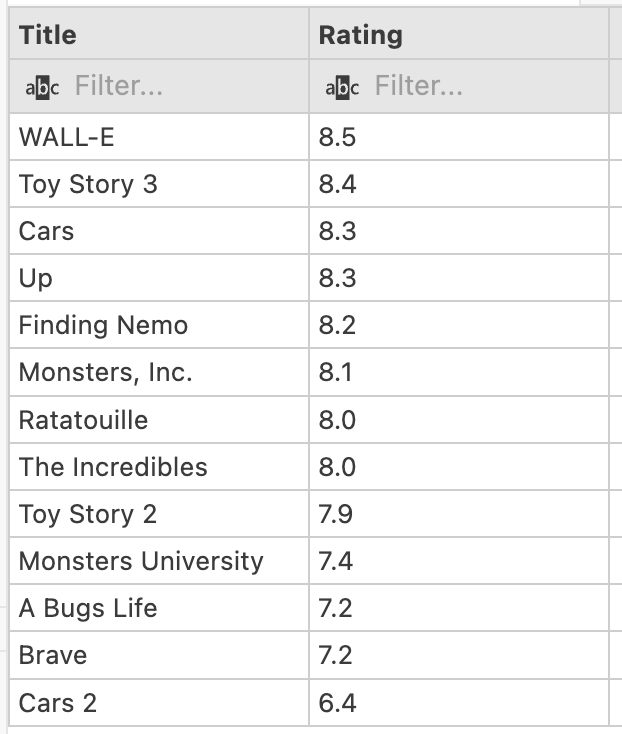
\includegraphics[width=.8\linewidth]{images/output/q7.png}
        \caption*{List of all the movies by their ratings in descending order.}
        \label{fig:q7}
    \end{subfigure}
    \begin{subfigure}{.5\textwidth}
        \centering
        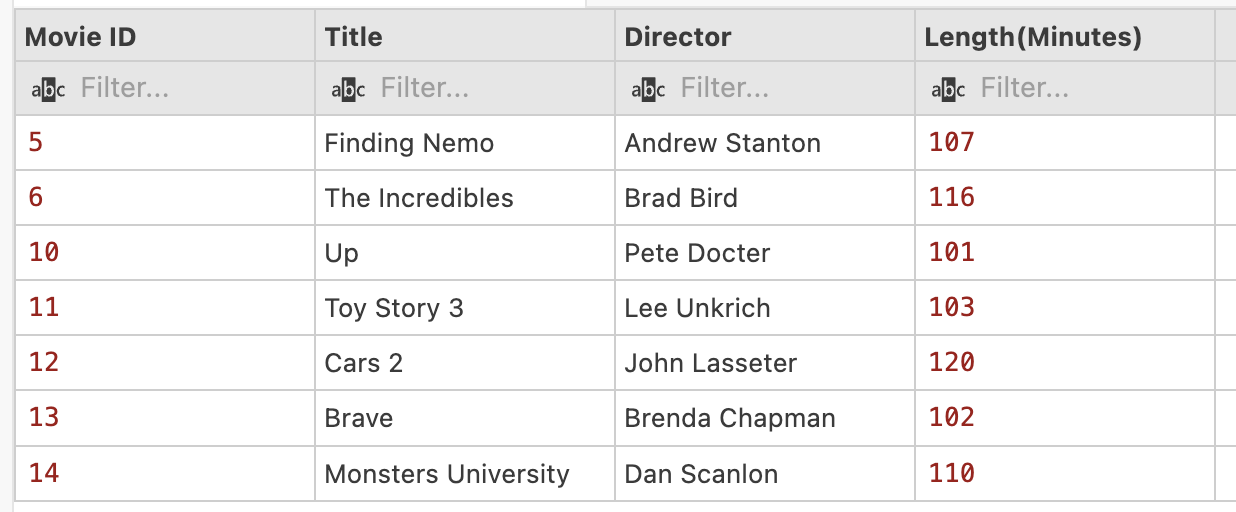
\includegraphics[width=.8\linewidth]{images/output/q8.png}
        \caption*{Movie ID, Name of the movies that the highest length movie of each director.}
        \label{fig:q8}
    \end{subfigure}
    \begin{subfigure}{\textwidth}
        \centering
        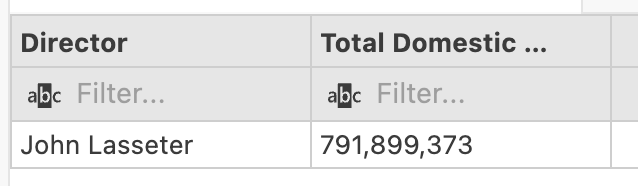
\includegraphics[width=.66\linewidth]{images/output/q9.png}
        \caption*{Local domestic sales of movies by John Lasseter so far.}
        \label{fig:q9}
    \end{subfigure}
\end{figure}
